\section{Qualitative Analysis}
\label{sec:experiments_qualitative_latent_space_analysis}

The metrics reported in Section~\ref{sec:experiments_latent_space_analysis} evaluate the \gls{ls} clusterings quantitatively but do not indicate what the resulting clusters actually represent.
This section complements them with a qualitative, hand-labeled inspection of the clusters obtained for each environment.

To select the clusterings for the qualitative analysis, several criteria are considered.
First, clusterings with very few clusters, such as two clusters, are excluded because they provide an overly coarse representation of the latent space.
The selected clustering should also achieve a sufficiently high \gls{acu}, indicating a good balance between consistency and abstraction.
Finally, the number of clusters must remain small enough to allow the resulting clusters to be examined manually.
These criteria provide a practical basis for selecting clusterings that are both quantitatively meaningful and suitable for qualitative analysis.

\newpage
\subsection{\BreakoutName}

\begin{figure}[H]
    \qualitativeClusterFigureSetup
    \qualitativeClusterTwo
        {figures/clustering_agent_representation/pictures/breakout/qualitative/cluster_0/image_1.png}
        {figures/clustering_agent_representation/pictures/breakout/qualitative/cluster_0/image_2.png}
        {C}
    \qualitativeClusterTwo
        {figures/clustering_agent_representation/pictures/breakout/qualitative/cluster_1/image_1.png}
        {figures/clustering_agent_representation/pictures/breakout/qualitative/cluster_1/image_2.png}
        {D}
    \qualitativeClusterTwo
        {figures/clustering_agent_representation/pictures/breakout/qualitative/cluster_2/image_1.png}
        {figures/clustering_agent_representation/pictures/breakout/qualitative/cluster_2/image_2.png}
        {E}
    \qualitativeClusterTwo
        {figures/clustering_agent_representation/pictures/breakout/qualitative/cluster_3/image_1.png}
        {figures/clustering_agent_representation/pictures/breakout/qualitative/cluster_3/image_2.png}
        {F}
    \qualitativeClusterTwo
        {figures/clustering_agent_representation/pictures/breakout/qualitative/cluster_4/image_1.png}
        {figures/clustering_agent_representation/pictures/breakout/qualitative/cluster_4/image_2.png}
        {G}
    \caption{Clusters C--G identified by \gls{car} in the \BreakoutName environment (layer 6b, $K=5$).}
    \label{fig:qualitative_breakout}
\end{figure}


Figure~\ref{fig:qualitative_breakout} shows the clusters obtained at layer 6b with $K=5$.
The clustering separates the beginning of the episode into three clusters distinguished mainly by the paddle's position, and isolates two more advanced game states, one in which the agent has dug a tunnel through the left side of the wall and one in which the ball is behind the wall.

\newpage
\subsection{\MarioBrosName}

\begin{figure}[H]
    \qualitativeClusterFigureSetup
    \qualitativeClusterTwo
        {figures/clustering_agent_representation/pictures/mario_bros/qualitative/cluster_0/image_1.png}
        {figures/clustering_agent_representation/pictures/mario_bros/qualitative/cluster_0/image_2.png}
        {A}
    \qualitativeClusterTwo
        {figures/clustering_agent_representation/pictures/mario_bros/qualitative/cluster_1/image_1.png}
        {figures/clustering_agent_representation/pictures/mario_bros/qualitative/cluster_1/image_2.png}
        {B}
    \qualitativeClusterTwo
        {figures/clustering_agent_representation/pictures/mario_bros/qualitative/cluster_2/image_1.png}
        {figures/clustering_agent_representation/pictures/mario_bros/qualitative/cluster_2/image_2.png}
        {C}
    \caption{Clusters A--C identified by \gls{car} in the \MarioBrosName environment (layer 3, $K=3$).}
    \label{fig:qualitative_mario_bros}
\end{figure}


Figure~\ref{fig:qualitative_mario_bros} shows the clusters obtained at layer 3 with $K=3$.
Rather than separating phases of the episode, the clustering separates the side of the screen on which Mario is fighting enemies, together with a third cluster corresponding to hitting the POW block, a fixed, recognizable location in the level.

\newpage
\subsection{\MsPacManName}

\begin{figure}[t]
    \centering
    \resizebox{\textwidth}{!}{
    \begin{tikzpicture}

    \node (ligne_1) at (0, 0) {};

    \node[] at ($(ligne_1) + (-4.5cm, 0cm)$) {
    \begin{minipage}{4.5cm}
        \centering
        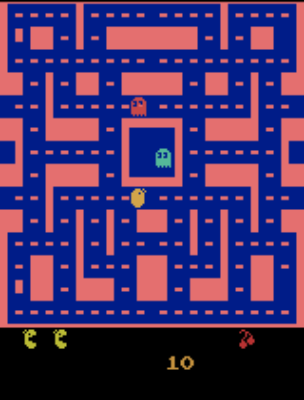
\includegraphics[width=2cm]{figures/clustering_agent_representation/pictures/ms_pacman/qualitative/cluster_1/image_1.png}
        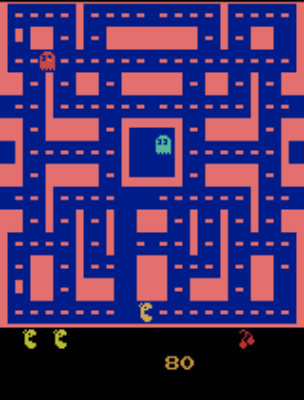
\includegraphics[width=2cm]{figures/clustering_agent_representation/pictures/ms_pacman/qualitative/cluster_1/image_2.png}

        \small Start of the episode.
    \end{minipage}
    };

    \node[] at ($(ligne_1) + (0cm, 0cm)$) {
    \begin{minipage}{4.5cm}
        \centering
        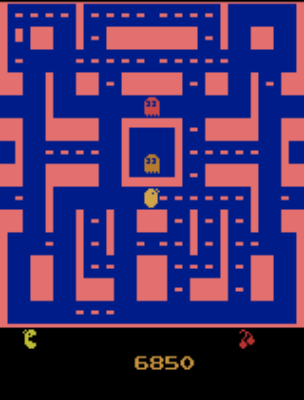
\includegraphics[width=2cm]{figures/clustering_agent_representation/pictures/ms_pacman/qualitative/cluster_0/image_1.png}
        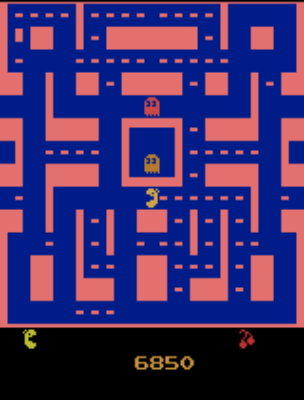
\includegraphics[width=2cm]{figures/clustering_agent_representation/pictures/ms_pacman/qualitative/cluster_0/image_2.png}

        \small Middle of the episode.
    \end{minipage}
    };

    \node[] at ($(ligne_1) + (4.5cm, 0cm)$) {
    \begin{minipage}{4.5cm}
        \centering
        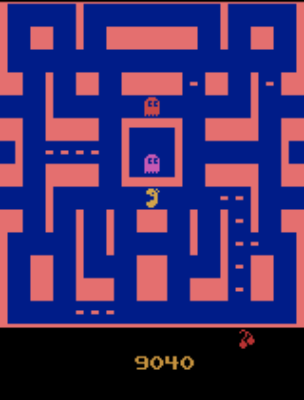
\includegraphics[width=2cm]{figures/clustering_agent_representation/pictures/ms_pacman/qualitative/cluster_2/image_1.png}
        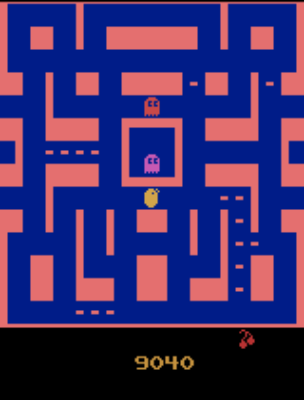
\includegraphics[width=2cm]{figures/clustering_agent_representation/pictures/ms_pacman/qualitative/cluster_2/image_2.png}

        \small End of the episode.
    \end{minipage}
    };

    \end{tikzpicture}
    }
    \caption{Clusters identified by \gls{car} in the Ms.\ Pac-Man environment (layer 6b, $K=3$).}
    \label{fig:qualitative_ms_pacman}
\end{figure}


Figure~\ref{fig:qualitative_ms_pacman} shows the clusters obtained at layer 6b with $K=3$.
Unlike \MarioBrosName, the clustering here separates the coarse temporal phase of the episode, tracked through the score and the number of pellets remaining in the maze, rather than a spatial feature of the observation.

\newpage
\subsection{\PongName}

\begin{figure}[H]
    \qualitativeClusterFigureSetup
    \qualitativeClusterTwo
        {figures/clustering_agent_representation/pictures/pong/qualitative/cluster_0/image_1.png}
        {figures/clustering_agent_representation/pictures/pong/qualitative/cluster_0/image_2.png}
        {Cluster 1: the ball is near the bottom of the field.}
    \qualitativeClusterTwo
        {figures/clustering_agent_representation/pictures/pong/qualitative/cluster_1/image_1.png}
        {figures/clustering_agent_representation/pictures/pong/qualitative/cluster_1/image_2.png}
        {Cluster 2: the ball crosses above the opponent's paddle, left behind at the bottom.}
    \qualitativeClusterTwo
        {figures/clustering_agent_representation/pictures/pong/qualitative/cluster_4/image_1.png}
        {figures/clustering_agent_representation/pictures/pong/qualitative/cluster_4/image_2.png}
        {Cluster 3: the ball is near the top of the field, close to the player's paddle.}
    \qualitativeClusterTwo
        {figures/clustering_agent_representation/pictures/pong/qualitative/cluster_2/image_1.png}
        {figures/clustering_agent_representation/pictures/pong/qualitative/cluster_2/image_2.png}
        {Cluster 4: same as cluster 1.}
    \qualitativeClusterTwo
        {figures/clustering_agent_representation/pictures/pong/qualitative/cluster_3/image_1.png}
        {figures/clustering_agent_representation/pictures/pong/qualitative/cluster_3/image_2.png}
        {Cluster 5: same as cluster 2.}
    \qualitativeClusterTwo
        {figures/clustering_agent_representation/pictures/pong/qualitative/cluster_5/image_1.png}
        {figures/clustering_agent_representation/pictures/pong/qualitative/cluster_5/image_2.png}
        {Cluster 6: same as cluster 3.}
    \caption{Clusters identified by \gls{car} in the \PongName environment (layer 4, $K=6$). Clusters 4--6 duplicate the semantics of clusters 1--3, illustrating over-segmentation at this value of $K$.}
    \label{fig:qualitative_pong}
\end{figure}


Figure~\ref{fig:qualitative_pong} shows the clusters obtained at layer 4 with $K=6$.
Inspection of the six clusters reveals only three distinct semantics, each split into two clusters: the ball near the bottom of the field, the ball crossing the court above the opponent's paddle left behind at the bottom, and the ball near the top of the field close to the player's paddle.
This is an instance of over-segmentation, in which increasing $K$ duplicates existing concepts instead of revealing new ones, consistent with the drop of \gls{cu} observed at high $K$ for this environment in Figure~\ref{fig:latent_space_curves_by_metric}.

\newpage
\subsection{\SpaceInvadersName}

\begin{figure}[H]
    \qualitativeClusterFigureSetup
    \qualitativeClusterTwo
        {figures/clustering_agent_representation/pictures/space_invaders/qualitative/cluster_3/image_1.png}
        {figures/clustering_agent_representation/pictures/space_invaders/qualitative/cluster_3/image_2.png}
        {Start of the episode.}
    \qualitativeClusterTwo
        {figures/clustering_agent_representation/pictures/space_invaders/qualitative/cluster_1/image_1.png}
        {figures/clustering_agent_representation/pictures/space_invaders/qualitative/cluster_1/image_2.png}
        {Middle of the episode.}
    \qualitativeClusterTwo
        {figures/clustering_agent_representation/pictures/space_invaders/qualitative/cluster_0/image_1.png}
        {figures/clustering_agent_representation/pictures/space_invaders/qualitative/cluster_0/image_2.png}
        {The left column has been cleared; the flying saucer occasionally appears.}
    \qualitativeClusterTwo
        {figures/clustering_agent_representation/pictures/space_invaders/qualitative/cluster_2/image_1.png}
        {figures/clustering_agent_representation/pictures/space_invaders/qualitative/cluster_2/image_2.png}
        {Late in the episode, few invaders remain.}
    \caption{Clusters identified by \gls{car} in the \SpaceInvadersName environment (layer 4, $K=4$).}
    \label{fig:qualitative_space_invaders}
\end{figure}


Figure~\ref{fig:qualitative_space_invaders} shows the clusters obtained at layer 4 with $K=4$.
Three clusters track the coarse progression of the episode, from the initial, intact formation of invaders to the sparse, late-game configurations, while the fourth isolates a more specific behavior in which the agent has cleared the leftmost column and is positioned to catch the flying saucer that occasionally crosses the top of the screen.

\newpage
\subsection{\SurroundName}

\begin{figure}[H]
    \qualitativeClusterFigureSetup
    \qualitativeClusterTwo
        {figures/clustering_agent_representation/pictures/surround/qualitative/cluster_1/image_1.png}
        {figures/clustering_agent_representation/pictures/surround/qualitative/cluster_1/image_2.png}
        {Start of the episode.}
    \qualitativeClusterTwo
        {figures/clustering_agent_representation/pictures/surround/qualitative/cluster_0/image_1.png}
        {figures/clustering_agent_representation/pictures/surround/qualitative/cluster_0/image_2.png}
        {The agent's trail remains confined to the bottom-left area.}
    \qualitativeClusterTwo
        {figures/clustering_agent_representation/pictures/surround/qualitative/cluster_2/image_1.png}
        {figures/clustering_agent_representation/pictures/surround/qualitative/cluster_2/image_2.png}
        {The agent moves along the top of the level, arriving from the left.}
    \qualitativeClusterTwo
        {figures/clustering_agent_representation/pictures/surround/qualitative/cluster_3/image_1.png}
        {figures/clustering_agent_representation/pictures/surround/qualitative/cluster_3/image_2.png}
        {The trail grows from the top-left toward the bottom, closing in on the final enclosure.}
    \caption{Clusters identified by \gls{car} in the \SurroundName environment (layer 8b, $K=4$).}
    \label{fig:qualitative_surround}
\end{figure}


Figure~\ref{fig:qualitative_surround} shows the clusters obtained at layer 8b with $K=4$.
Besides the start of the episode, the clustering separates configurations by the region of the level occupied by the agent's trail, from a small trail confined to the bottom-left, to one running along the top after arriving from the left, to a dense trail that has grown from the top-left toward the bottom and is closing in on the final enclosure between the two players.

\newpage
